\chapter{DATA DAN METODOLOGI}
\vspace{1ex}

\section*{}
Penelitian ini dilaksanakan sesuai dengan desain sistem berikut dengan implementasinya. Desain sistem merupakan konsep dari pembuatan dan perancangan infrastruktur kemudian diwujudkan dalam bentuk blok-blok alur yang harus dikerjakan. Pada bagian implementasi merupakan pelaksanaan teknis untuk setiap blok pada desain sistem.
\vspace{1ex}

\section{Cakupan Tugas Akhir}
\vspace{1ex}

Tugas akhir ini merupakan salah satu bentuk implementasi Lightweight Convolutional Neural Network untuk melakukan pencarian seorang individu menggunakan gambar multi-modal berupa sketsa sebagai input, berikut pada Gambar 3.1 adalah cakupan Tugas Akhir dari Desain Sistem.
\begin{figure}  [!htb]
	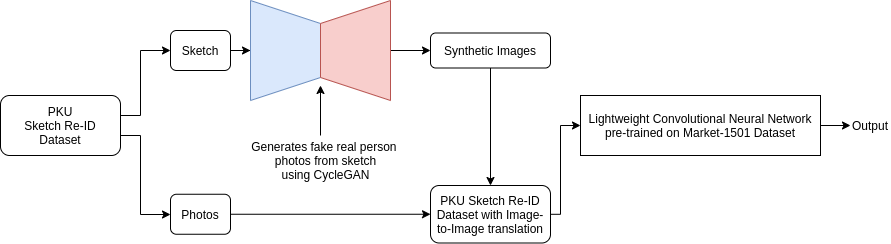
\includegraphics[scale=0.35]{img/desain_sistem.png}
	\caption{Desain Sistem}
	\label{fig: 3_1}
\end{figure}
\vspace{1ex}

\section{Penyesuaian Dataset PKU Sketch Re-ID}
Desain sistem secara umum pada gambar \ref{fig: 3_1}, yang mencakup beberapa hal, salah satunya ialah penyesuaian dataset. Dataset yang kami akan gunakan adalah dataset PKU Sketch Re-ID yang dibuat oleh Lu Pang \cite{cit:15}. Dataset ini terdiri dari 200 identitas yang unik, dimana setiap identitas telah ditangkap oleh dua kamera berbeda. Selain itu setiap individu memiliki satu gambar sketsa, sehingga seluruh dataset bertotal 600 gambar. Gambar \ref{fig: 3_2} menunjukkan beberapa contoh dari dataset PKU Sketch Re-ID. 

\begin{figure}  [!htb]
	\centering
	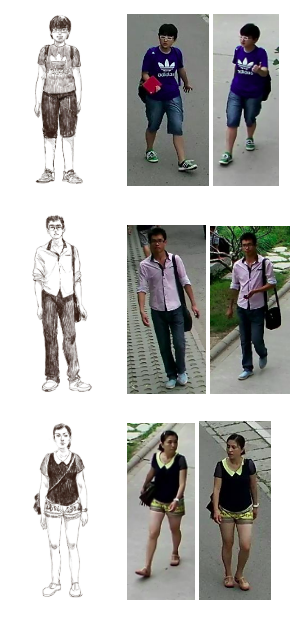
\includegraphics[scale=0.35]{img/ExamplesSketchReID.png}
	\caption{Beberapa contoh gambar pada Dataset PKU Sketch Re-ID}
	\label{fig: 3_2}
\end{figure}

Dataset PKU Sketch \cite{cit:15} Re-id kemudian akan melalui proses persiapan terlebih dahulu sehingga dapat dilakukan evaluasi performa dari Lightweight Convolutional Neural Network yang akan digunakan. Penyesuaian yang akan dilakukan pada dataset meliputi, penggabungan individu-individu sama yang tertangkap oleh kamera kamera berbeda, kemudian pemasangan individu tersebut ke gambar sketsa sehingga setiap individu unik akan menjadi kelas tersendiri. Kemudian dataset tersebut akan dibagi menjadi 150 identitas untuk training dan 50 identitas untuk testing, seperti yang ditunjukan pada gambar \ref{fig: 3_3}. Setiap gambar telah di \textit{crop} secara \textit{manual} untuk memastikan setiap gambar dari dataset hanya berisi satu individu yang spesifik. Untuk gambar sketsa yang digunakan, terdapat 5 orang seniman berbeda yang memiliki 5 \textit{art style} yang berbeda pula untuk menggambar masing masing identitas. 

\begin{figure}  [!htb]
	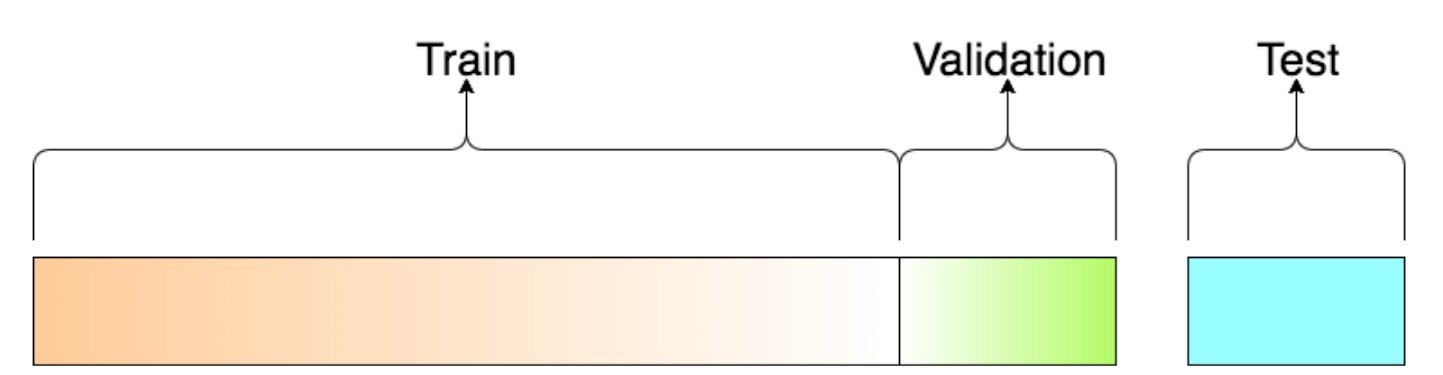
\includegraphics[scale=0.35]{img/dataset.png}
	\caption{Pembagian Dataset PKU Sketch Re-ID}
	\label{fig: 3_3}
\end{figure}

\section{Lightweight Convolutional Neural Network}
Setelah penyesuaian dataset telah dilakukan, akan dilakukan training dengan menggunakan Lightweight Residual Network yang pernah digunakan untuk memecahkan masalah klasifikasi CIFAR-10. Namun pada model yang kami gunakan, \textit{Fully-Connected Layer} terakhir dihilangkan, dan ditambahkan dua layer baru untuk menggantikan layer tersebut sehingga model dapat dipastikan akan mempelajari fitur-fitur yang terdapat pada dataset PKU Sketch Re-ID. Digunakan dua buah Fully-Connected layer supaya pada Fully Connected layer pertama dapat dilakukan pengenalan fitur diskriminan dari masing-masing individu, dan pada layer kedua dilakukan klasifikasi dari masing-masing individu tersebut. Selain itu, berbeda dengan model ResNet aslinya, model yang kami gunakan menggunakan resolusi input sebesar 32x64x3.

\begin{table}[h!]
	\begin{center}
		\begin{tabular}{|c|c|}
			\hline
			\textbf{Nama} & \textbf{Parameter} \\ \hline
			ResNet 56 & 0.85M \\ \hline
			ResNet 110 & 1.7M \\ \hline
			GoogleNet & 7M \\ \hline
			DenseNet121 & 8.6M \\ \hline
			ResNet 50 & 23M \\ \hline
		\end{tabular}
	\end{center}
	\vspace{1ex}
	\caption{Jumlah parameter untuk beberapa model popular.}
	\label{tabel:2}
\end{table}

Pada percobaan-percobaan yang kami lakukan, kami menggunakan tiga model Residual Network yang berbeda, yaitu ResNet 20, ResNet 56, dan ResNet 110. Namun kami hanya melanjutkan menggunakan ResNet 56 dan ResNet 110 dikarenakan kedua model tersebut mendapatkan hasil yang jauh lebih baik dibandingkan dengan pada ResNet 20. Meskipun layer dari kedua model yang kami gunakan relatif cukup dalam (56 dan 110 layer) apabila dibandingkan dengan Residual Network normalnya. Parameter yang terdapat pada model ini jauh lebih sedikit, dimana ResNet 110 hanya memiliki 1.7 juta parameter, jauh dari jutaan parameter yang dimiliki model-model populer seperti DenseNet, GoogleNet, dan ResNet 50.Pada tabel \ref{tab:long} dapat dilihat bentuk susunan layer dari ResNet 20 sendiri. Untuk susunan model ResNet 56 dapat dilihat pada \ref{tab:long2} dan untuk ResNet 110 dapat dilihat pada \ref{tab:long3}.

\begin{center}
	\begin{longtable}{|l|l|l|l|}
		\caption{Susunan Model ResNet 20} \label{tab:long} \\
		
		\hline \multicolumn{1}{|c|}{\textbf{Type}} & \multicolumn{1}{c|}{\textbf{Channel}} & \multicolumn{1}{c|}{\textbf{Size}} & \multicolumn{1}{c|}{\textbf{Stride}}\\ \hline 
		\endfirsthead
		
		\multicolumn{4}{c}%
		{{\bfseries \tablename\ \thetable{} -- Dilanjutkan dari halaman sebelumnya}} \\
		\hline \multicolumn{1}{|c|}{\textbf{Type}} & \multicolumn{1}{c|}{\textbf{Channel}} & \multicolumn{1}{c|}{\textbf{Size}} & \multicolumn{1}{c|}{\textbf{Stride}}\\ \hline 
		\endhead
		
		\hline \multicolumn{4}{|r|}{{Dilanjutkan ke halaman selanjutnya}} \\ \hline
		\endfoot
		
		\hline \hline
		\endlastfoot
		Convolutional2D & 16 & 3x3 & 1x1 \\
		BatchNorm2D & 16 & \_ & \_ \\ 
		Convolutional2D & 16 & 3x3 & 1x1 \\
		BatchNorm2D & 16 & \_ & \_ \\
		Convolutional2D & 16 & 3x3 & 1x1 \\
		BatchNorm2D & 16 & \_ & \_ \\
		Convolutional2D & 16 & 3x3 & 1x1 \\
		BatchNorm2D & 16 & \_ & \_ \\
		Convolutional2D & 16 & 3x3 & 1x1 \\
		BatchNorm2D & 16 & \_ & \_ \\
		Convolutional2D & 16 & 3x3 & 1x1 \\
		BatchNorm2D & 16 & \_ & \_ \\
		Convolutional2D & 16 & 3x3 & 1x1 \\
		BatchNorm2D & 16 & \_ & \_ \\
		Convolutional2D & 32 & 3x3 & 2x2 \\
		BatchNorm2D & 32 & \_ & \_ \\
		Convolutional2D & 32 & 3x3 & 1x1 \\
		BatchNorm2D & 32 & \_ & \_ \\
		Convolutional2D & 32 & 3x3 & 1x1 \\
		BatchNorm2D & 32 & \_ & \_ \\
		Convolutional2D & 32 & 3x3 & 1x1 \\
		BatchNorm2D & 32 & \_ & \_ \\
		Convolutional2D & 32 & 3x3 & 1x1 \\
		BatchNorm2D & 32 & \_ & \_ \\
		Convolutional2D & 32 & 3x3 & 1x1 \\
		BatchNorm2D & 32 & \_ & \_ \\
		Convolutional2D & 64 & 3x3 & 2x2 \\
		BatchNorm2D & 64 & \_ & \_ \\
		Convolutional2D & 64 & 3x3 & 1x1 \\
		BatchNorm2D & 64 & \_ & \_ \\
		Convolutional2D & 64 & 3x3 & 1x1 \\
		BatchNorm2D & 64 & \_ & \_ \\
		Convolutional2D & 64 & 3x3 & 1x1 \\
		BatchNorm2D & 64 & \_ & \_ \\
		Convolutional2D & 64 & 3x3 & 1x1 \\
		BatchNorm2D & 64 & \_ & \_ \\
		Convolutional2D & 64 & 3x3 & 1x1 \\
		BatchNorm2D & 64 & \_ & \_ \\
		FullyConnected & \_ & \_ & \_ \\
		BatchNorm1D & 512 & \_ & \_ \\
		Dropout & \_ & \_ & \_ \\
		FullyConnected & \_ & \_ & \_ \\
	\end{longtable}
\end{center}

\begin{center}
	\begin{longtable}{|l|l|l|l|}
		\caption{Susunan Model ResNet 56} \label{tab:long2} \\
		
		\hline \multicolumn{1}{|c|}{\textbf{Type}} & \multicolumn{1}{c|}{\textbf{Channel}} & \multicolumn{1}{c|}{\textbf{Size}} & \multicolumn{1}{c|}{\textbf{Stride}}\\ \hline 
		\endfirsthead
		
		\multicolumn{4}{c}%
		{{\bfseries \tablename\ \thetable{} -- Dilanjutkan dari halaman sebelumnya}} \\
		\hline \multicolumn{1}{|c|}{\textbf{Type}} & \multicolumn{1}{c|}{\textbf{Channel}} & \multicolumn{1}{c|}{\textbf{Size}} & \multicolumn{1}{c|}{\textbf{Stride}}\\ \hline 
		\endhead
		
		\hline \multicolumn{4}{|r|}{{Dilanjutkan ke halaman selanjutnya}} \\ \hline
		\endfoot
		
		\hline \hline
		\endlastfoot
		Convolutional2D & 16 & 3x3 & 1x1 \\
		BatchNorm2D & 16 & \_ & \_ \\ 
		Convolutional2D & 16 & 3x3 & 1x1 \\
		BatchNorm2D & 16 & \_ & \_ \\
		Convolutional2D & 16 & 3x3 & 1x1 \\
		BatchNorm2D & 16 & \_ & \_ \\
		Convolutional2D & 16 & 3x3 & 1x1 \\
		BatchNorm2D & 16 & \_ & \_ \\
		Convolutional2D & 16 & 3x3 & 1x1 \\
		BatchNorm2D & 16 & \_ & \_ \\
		Convolutional2D & 16 & 3x3 & 1x1 \\
		BatchNorm2D & 16 & \_ & \_ \\
		Convolutional2D & 16 & 3x3 & 1x1 \\
		BatchNorm2D & 16 & \_ & \_ \\
		Convolutional2D & 16 & 3x3 & 1x1 \\
		BatchNorm2D & 16 & \_ & \_ \\
		Convolutional2D & 16 & 3x3 & 1x1 \\
		BatchNorm2D & 16 & \_ & \_ \\
		Convolutional2D & 16 & 3x3 & 1x1 \\
		BatchNorm2D & 16 & \_ & \_ \\
		Convolutional2D & 16 & 3x3 & 1x1 \\
		BatchNorm2D & 16 & \_ & \_ \\
		Convolutional2D & 16 & 3x3 & 1x1 \\
		BatchNorm2D & 16 & \_ & \_ \\
		Convolutional2D & 16 & 3x3 & 1x1 \\
		BatchNorm2D & 16 & \_ & \_ \\
		Convolutional2D & 16 & 3x3 & 1x1 \\
		BatchNorm2D & 16 & \_ & \_ \\
		Convolutional2D & 16 & 3x3 & 1x1 \\
		BatchNorm2D & 16 & \_ & \_ \\
		Convolutional2D & 16 & 3x3 & 1x1 \\
		BatchNorm2D & 16 & \_ & \_ \\
		Convolutional2D & 16 & 3x3 & 1x1 \\
		BatchNorm2D & 16 & \_ & \_ \\
		Convolutional2D & 16 & 3x3 & 1x1 \\
		BatchNorm2D & 16 & \_ & \_ \\
		Convolutional2D & 16 & 3x3 & 1x1 \\
		BatchNorm2D & 16 & \_ & \_ \\
		Convolutional2D & 32 & 3x3 & 2x2 \\
		BatchNorm2D & 32 & \_ & \_ \\
		Convolutional2D & 32 & 3x3 & 1x1 \\
		BatchNorm2D & 32 & \_ & \_ \\
		Convolutional2D & 32 & 3x3 & 1x1 \\
		BatchNorm2D & 32 & \_ & \_ \\
		Convolutional2D & 32 & 3x3 & 1x1 \\
		BatchNorm2D & 32 & \_ & \_ \\
		Convolutional2D & 32 & 3x3 & 1x1 \\
		BatchNorm2D & 32 & \_ & \_ \\
		Convolutional2D & 32 & 3x3 & 1x1 \\
		BatchNorm2D & 32 & \_ & \_ \\
		Convolutional2D & 32 & 3x3 & 1x1 \\
		BatchNorm2D & 32 & \_ & \_ \\
		Convolutional2D & 32 & 3x3 & 1x1 \\
		BatchNorm2D & 32 & \_ & \_ \\
		Convolutional2D & 32 & 3x3 & 1x1 \\
		BatchNorm2D & 32 & \_ & \_ \\
		Convolutional2D & 32 & 3x3 & 1x1 \\
		BatchNorm2D & 32 & \_ & \_ \\
		Convolutional2D & 32 & 3x3 & 1x1 \\
		BatchNorm2D & 32 & \_ & \_ \\
		Convolutional2D & 32 & 3x3 & 1x1 \\
		BatchNorm2D & 32 & \_ & \_ \\
		Convolutional2D & 32 & 3x3 & 1x1 \\
		BatchNorm2D & 32 & \_ & \_ \\
		Convolutional2D & 32 & 3x3 & 1x1 \\
		BatchNorm2D & 32 & \_ & \_ \\
		Convolutional2D & 32 & 3x3 & 1x1 \\
		BatchNorm2D & 32 & \_ & \_ \\
		Convolutional2D & 32 & 3x3 & 1x1 \\
		BatchNorm2D & 32 & \_ & \_ \\
		Convolutional2D & 32 & 3x3 & 1x1 \\
		BatchNorm2D & 32 & \_ & \_ \\
		Convolutional2D & 32 & 3x3 & 1x1 \\
		BatchNorm2D & 32 & \_ & \_ \\
		Convolutional2D & 64 & 3x3 & 2x2 \\
		BatchNorm2D & 64 & \_ & \_ \\
		Convolutional2D & 64 & 3x3 & 1x1 \\
		BatchNorm2D & 64 & \_ & \_ \\
		Convolutional2D & 64 & 3x3 & 1x1 \\
		BatchNorm2D & 64 & \_ & \_ \\
		Convolutional2D & 64 & 3x3 & 1x1 \\
		BatchNorm2D & 64 & \_ & \_ \\
		Convolutional2D & 64 & 3x3 & 1x1 \\
		BatchNorm2D & 64 & \_ & \_ \\
		Convolutional2D & 64 & 3x3 & 1x1 \\
		BatchNorm2D & 64 & \_ & \_ \\
		Convolutional2D & 64 & 3x3 & 1x1 \\
		BatchNorm2D & 64 & \_ & \_ \\
		Convolutional2D & 64 & 3x3 & 1x1 \\
		BatchNorm2D & 64 & \_ & \_ \\
		Convolutional2D & 64 & 3x3 & 1x1 \\
		BatchNorm2D & 64 & \_ & \_ \\
		Convolutional2D & 64 & 3x3 & 1x1 \\
		BatchNorm2D & 64 & \_ & \_ \\
		Convolutional2D & 64 & 3x3 & 1x1 \\
		BatchNorm2D & 64 & \_ & \_ \\
		Convolutional2D & 64 & 3x3 & 1x1 \\
		BatchNorm2D & 64 & \_ & \_ \\
		Convolutional2D & 64 & 3x3 & 1x1 \\
		BatchNorm2D & 64 & \_ & \_ \\
		Convolutional2D & 64 & 3x3 & 1x1 \\
		BatchNorm2D & 64 & \_ & \_ \\
		Convolutional2D & 64 & 3x3 & 1x1 \\
		BatchNorm2D & 64 & \_ & \_ \\
		Convolutional2D & 64 & 3x3 & 1x1 \\
		BatchNorm2D & 64 & \_ & \_ \\
		Convolutional2D & 64 & 3x3 & 1x1 \\
		BatchNorm2D & 64 & \_ & \_ \\
		Convolutional2D & 64 & 3x3 & 1x1 \\
		BatchNorm2D & 64 & \_ & \_ \\
		FullyConnected & \_ & \_ & \_ \\
		BatchNorm1D & 512 & \_ & \_ \\
		Dropout & \_ & \_ & \_ \\
		FullyConnected & \_ & \_ & \_ \\
	\end{longtable}
\end{center}

\begin{center}
	\begin{longtable}{|l|l|l|l|}
		\caption{Susunan Model ResNet 110} \label{tab:long3} \\
		
		\hline \multicolumn{1}{|c|}{\textbf{Type}} & \multicolumn{1}{c|}{\textbf{Channel}} & \multicolumn{1}{c|}{\textbf{Size}} & \multicolumn{1}{c|}{\textbf{Stride}}\\ \hline 
		\endfirsthead
		
		\multicolumn{4}{c}%
		{{\bfseries \tablename\ \thetable{} -- Dilanjutkan dari halaman sebelumnya}} \\
		\hline \multicolumn{1}{|c|}{\textbf{Type}} & \multicolumn{1}{c|}{\textbf{Channel}} & \multicolumn{1}{c|}{\textbf{Size}} & \multicolumn{1}{c|}{\textbf{Stride}}\\ \hline 
		\endhead
		
		\hline \multicolumn{4}{|r|}{{Dilanjutkan ke halaman selanjutnya}} \\ \hline
		\endfoot
		
		\hline \hline
		\endlastfoot
		Convolutional2D & 16 & 3x3 & 1x1 \\
		BatchNorm2D & 16 & \_ & \_ \\ 
		Convolutional2D & 16 & 3x3 & 1x1 \\
		BatchNorm2D & 16 & \_ & \_ \\
		Convolutional2D & 16 & 3x3 & 1x1 \\
		BatchNorm2D & 16 & \_ & \_ \\
		Convolutional2D & 16 & 3x3 & 1x1 \\
		BatchNorm2D & 16 & \_ & \_ \\
		Convolutional2D & 16 & 3x3 & 1x1 \\
		BatchNorm2D & 16 & \_ & \_ \\
		Convolutional2D & 16 & 3x3 & 1x1 \\
		BatchNorm2D & 16 & \_ & \_ \\
		Convolutional2D & 16 & 3x3 & 1x1 \\
		BatchNorm2D & 16 & \_ & \_ \\
		Convolutional2D & 16 & 3x3 & 1x1 \\
		BatchNorm2D & 16 & \_ & \_ \\
		Convolutional2D & 16 & 3x3 & 1x1 \\
		BatchNorm2D & 16 & \_ & \_ \\
		Convolutional2D & 16 & 3x3 & 1x1 \\
		BatchNorm2D & 16 & \_ & \_ \\
		Convolutional2D & 16 & 3x3 & 1x1 \\
		BatchNorm2D & 16 & \_ & \_ \\
		Convolutional2D & 16 & 3x3 & 1x1 \\
		BatchNorm2D & 16 & \_ & \_ \\
		Convolutional2D & 16 & 3x3 & 1x1 \\
		BatchNorm2D & 16 & \_ & \_ \\
		Convolutional2D & 16 & 3x3 & 1x1 \\
		BatchNorm2D & 16 & \_ & \_ \\
		Convolutional2D & 16 & 3x3 & 1x1 \\
		BatchNorm2D & 16 & \_ & \_ \\
		Convolutional2D & 16 & 3x3 & 1x1 \\
		BatchNorm2D & 16 & \_ & \_ \\
		Convolutional2D & 16 & 3x3 & 1x1 \\
		BatchNorm2D & 16 & \_ & \_ \\
		Convolutional2D & 16 & 3x3 & 1x1 \\
		BatchNorm2D & 16 & \_ & \_ \\
		Convolutional2D & 16 & 3x3 & 1x1 \\
		BatchNorm2D & 16 & \_ & \_ \\
		Convolutional2D & 16 & 3x3 & 1x1 \\
		BatchNorm2D & 16 & \_ & \_ \\
		Convolutional2D & 16 & 3x3 & 1x1 \\
		BatchNorm2D & 16 & \_ & \_ \\
		Convolutional2D & 16 & 3x3 & 1x1 \\
		BatchNorm2D & 16 & \_ & \_ \\
		Convolutional2D & 16 & 3x3 & 1x1 \\
		BatchNorm2D & 16 & \_ & \_ \\
		Convolutional2D & 16 & 3x3 & 1x1 \\
		BatchNorm2D & 16 & \_ & \_ \\
		Convolutional2D & 16 & 3x3 & 1x1 \\
		BatchNorm2D & 16 & \_ & \_ \\
		Convolutional2D & 16 & 3x3 & 1x1 \\
		BatchNorm2D & 16 & \_ & \_ \\
		Convolutional2D & 16 & 3x3 & 1x1 \\
		BatchNorm2D & 16 & \_ & \_ \\
		Convolutional2D & 16 & 3x3 & 1x1 \\
		BatchNorm2D & 16 & \_ & \_ \\
		Convolutional2D & 16 & 3x3 & 1x1 \\
		BatchNorm2D & 16 & \_ & \_ \\
		Convolutional2D & 16 & 3x3 & 1x1 \\
		BatchNorm2D & 16 & \_ & \_ \\
		Convolutional2D & 16 & 3x3 & 1x1 \\
		BatchNorm2D & 16 & \_ & \_ \\
		Convolutional2D & 16 & 3x3 & 1x1 \\
		BatchNorm2D & 16 & \_ & \_ \\
		Convolutional2D & 16 & 3x3 & 1x1 \\
		BatchNorm2D & 16 & \_ & \_ \\
		Convolutional2D & 16 & 3x3 & 1x1 \\
		BatchNorm2D & 16 & \_ & \_ \\
		Convolutional2D & 16 & 3x3 & 1x1 \\
		BatchNorm2D & 16 & \_ & \_ \\
		Convolutional2D & 16 & 3x3 & 1x1 \\
		BatchNorm2D & 16 & \_ & \_ \\
		Convolutional2D & 16 & 3x3 & 1x1 \\
		BatchNorm2D & 16 & \_ & \_ \\
		Convolutional2D & 32 & 3x3 & 2x2 \\
		BatchNorm2D & 32 & \_ & \_ \\
		Convolutional2D & 32 & 3x3 & 1x1 \\
		BatchNorm2D & 32 & \_ & \_ \\
		Convolutional2D & 32 & 3x3 & 1x1 \\
		BatchNorm2D & 32 & \_ & \_ \\
		Convolutional2D & 32 & 3x3 & 1x1 \\
		BatchNorm2D & 32 & \_ & \_ \\
		Convolutional2D & 32 & 3x3 & 1x1 \\
		BatchNorm2D & 32 & \_ & \_ \\
		Convolutional2D & 32 & 3x3 & 1x1 \\
		BatchNorm2D & 32 & \_ & \_ \\
		Convolutional2D & 32 & 3x3 & 1x1 \\
		BatchNorm2D & 32 & \_ & \_ \\
		Convolutional2D & 32 & 3x3 & 1x1 \\
		BatchNorm2D & 32 & \_ & \_ \\
		Convolutional2D & 32 & 3x3 & 1x1 \\
		BatchNorm2D & 32 & \_ & \_ \\
		Convolutional2D & 32 & 3x3 & 1x1 \\
		BatchNorm2D & 32 & \_ & \_ \\
		Convolutional2D & 32 & 3x3 & 1x1 \\
		BatchNorm2D & 32 & \_ & \_ \\
		Convolutional2D & 32 & 3x3 & 1x1 \\
		BatchNorm2D & 32 & \_ & \_ \\
		Convolutional2D & 32 & 3x3 & 1x1 \\
		BatchNorm2D & 32 & \_ & \_ \\
		Convolutional2D & 32 & 3x3 & 1x1 \\
		BatchNorm2D & 32 & \_ & \_ \\
		Convolutional2D & 32 & 3x3 & 1x1 \\
		BatchNorm2D & 32 & \_ & \_ \\
		Convolutional2D & 32 & 3x3 & 1x1 \\
		BatchNorm2D & 32 & \_ & \_ \\
		Convolutional2D & 32 & 3x3 & 1x1 \\
		BatchNorm2D & 32 & \_ & \_ \\
		Convolutional2D & 32 & 3x3 & 1x1 \\
		BatchNorm2D & 32 & \_ & \_ \\
		Convolutional2D & 32 & 3x3 & 1x1 \\
		BatchNorm2D & 32 & \_ & \_ \\
		Convolutional2D & 32 & 3x3 & 1x1 \\
		BatchNorm2D & 32 & \_ & \_ \\
		Convolutional2D & 32 & 3x3 & 1x1 \\
		BatchNorm2D & 32 & \_ & \_ \\
		Convolutional2D & 32 & 3x3 & 1x1 \\
		BatchNorm2D & 32 & \_ & \_ \\
		Convolutional2D & 32 & 3x3 & 1x1 \\
		BatchNorm2D & 32 & \_ & \_ \\
		Convolutional2D & 32 & 3x3 & 1x1 \\
		BatchNorm2D & 32 & \_ & \_ \\
		Convolutional2D & 32 & 3x3 & 1x1 \\
		BatchNorm2D & 32 & \_ & \_ \\
		Convolutional2D & 32 & 3x3 & 1x1 \\
		BatchNorm2D & 32 & \_ & \_ \\
		Convolutional2D & 32 & 3x3 & 1x1 \\
		BatchNorm2D & 32 & \_ & \_ \\
		Convolutional2D & 32 & 3x3 & 1x1 \\
		BatchNorm2D & 32 & \_ & \_ \\
		Convolutional2D & 32 & 3x3 & 1x1 \\
		BatchNorm2D & 32 & \_ & \_ \\
		Convolutional2D & 32 & 3x3 & 1x1 \\
		BatchNorm2D & 32 & \_ & \_ \\
		Convolutional2D & 32 & 3x3 & 1x1 \\
		BatchNorm2D & 32 & \_ & \_ \\
		Convolutional2D & 32 & 3x3 & 1x1 \\
		BatchNorm2D & 32 & \_ & \_ \\
		Convolutional2D & 32 & 3x3 & 1x1 \\
		BatchNorm2D & 32 & \_ & \_ \\
		Convolutional2D & 32 & 3x3 & 1x1 \\
		BatchNorm2D & 32 & \_ & \_ \\
		Convolutional2D & 32 & 3x3 & 1x1 \\
		BatchNorm2D & 32 & \_ & \_ \\
		Convolutional2D & 32 & 3x3 & 1x1 \\
		BatchNorm2D & 32 & \_ & \_ \\
		Convolutional2D & 64 & 3x3 & 2x2 \\
		BatchNorm2D & 64 & \_ & \_ \\
		Convolutional2D & 64 & 3x3 & 1x1 \\
		BatchNorm2D & 64 & \_ & \_ \\
		Convolutional2D & 64 & 3x3 & 1x1 \\
		BatchNorm2D & 64 & \_ & \_ \\
		Convolutional2D & 64 & 3x3 & 1x1 \\
		BatchNorm2D & 64 & \_ & \_ \\
		Convolutional2D & 64 & 3x3 & 1x1 \\
		BatchNorm2D & 64 & \_ & \_ \\
		Convolutional2D & 64 & 3x3 & 1x1 \\
		BatchNorm2D & 64 & \_ & \_ \\
		Convolutional2D & 64 & 3x3 & 1x1 \\
		BatchNorm2D & 64 & \_ & \_ \\
		Convolutional2D & 64 & 3x3 & 1x1 \\
		BatchNorm2D & 64 & \_ & \_ \\
		Convolutional2D & 64 & 3x3 & 1x1 \\
		BatchNorm2D & 64 & \_ & \_ \\
		Convolutional2D & 64 & 3x3 & 1x1 \\
		BatchNorm2D & 64 & \_ & \_ \\
		Convolutional2D & 64 & 3x3 & 1x1 \\
		BatchNorm2D & 64 & \_ & \_ \\
		Convolutional2D & 64 & 3x3 & 1x1 \\
		BatchNorm2D & 64 & \_ & \_ \\
		Convolutional2D & 64 & 3x3 & 1x1 \\
		BatchNorm2D & 64 & \_ & \_ \\
		Convolutional2D & 64 & 3x3 & 1x1 \\
		BatchNorm2D & 64 & \_ & \_ \\
		Convolutional2D & 64 & 3x3 & 1x1 \\
		BatchNorm2D & 64 & \_ & \_ \\
		Convolutional2D & 64 & 3x3 & 1x1 \\
		BatchNorm2D & 64 & \_ & \_ \\
		Convolutional2D & 64 & 3x3 & 1x1 \\
		BatchNorm2D & 64 & \_ & \_ \\
		Convolutional2D & 64 & 3x3 & 1x1 \\
		BatchNorm2D & 64 & \_ & \_ \\
		Convolutional2D & 64 & 3x3 & 1x1 \\
		BatchNorm2D & 64 & \_ & \_ \\
		Convolutional2D & 64 & 3x3 & 1x1 \\
		BatchNorm2D & 64 & \_ & \_ \\
		Convolutional2D & 64 & 3x3 & 1x1 \\
		BatchNorm2D & 64 & \_ & \_ \\
		Convolutional2D & 64 & 3x3 & 1x1 \\
		BatchNorm2D & 64 & \_ & \_ \\
		Convolutional2D & 64 & 3x3 & 1x1 \\
		BatchNorm2D & 64 & \_ & \_ \\
		Convolutional2D & 64 & 3x3 & 1x1 \\
		BatchNorm2D & 64 & \_ & \_ \\
		Convolutional2D & 64 & 3x3 & 1x1 \\
		BatchNorm2D & 64 & \_ & \_ \\
		Convolutional2D & 64 & 3x3 & 1x1 \\
		BatchNorm2D & 64 & \_ & \_ \\
		Convolutional2D & 64 & 3x3 & 1x1 \\
		BatchNorm2D & 64 & \_ & \_ \\
		Convolutional2D & 64 & 3x3 & 1x1 \\
		BatchNorm2D & 64 & \_ & \_ \\
		Convolutional2D & 64 & 3x3 & 1x1 \\
		BatchNorm2D & 64 & \_ & \_ \\
		Convolutional2D & 64 & 3x3 & 1x1 \\
		BatchNorm2D & 64 & \_ & \_ \\
		Convolutional2D & 64 & 3x3 & 1x1 \\
		BatchNorm2D & 64 & \_ & \_ \\
		Convolutional2D & 64 & 3x3 & 1x1 \\
		BatchNorm2D & 64 & \_ & \_ \\
		Convolutional2D & 64 & 3x3 & 1x1 \\
		BatchNorm2D & 64 & \_ & \_ \\
		Convolutional2D & 64 & 3x3 & 1x1 \\
		BatchNorm2D & 64 & \_ & \_ \\
		Convolutional2D & 64 & 3x3 & 1x1 \\
		BatchNorm2D & 64 & \_ & \_ \\
		Convolutional2D & 64 & 3x3 & 1x1 \\
		BatchNorm2D & 64 & \_ & \_ \\
		FullyConnected & \_ & \_ & \_ \\
		BatchNorm1D & 512 & \_ & \_ \\
		Dropout & \_ & \_ & \_ \\
		FullyConnected & \_ & \_ & \_ \\
	\end{longtable}
\end{center}


\section{\textit{Cross Domain Image-to-Image Translation}}
\vspace{1ex}
Dikarenakan fitur yang dapat dikenali oleh model untuk membantu membedakan satu individu dengan yang lainnya sangat sedikit, maka digunakan \textit{image-to-image translation}, atau lebih spesifik CycleGAN. Penggunaan CycleGAN dapat menjembatani antara modalitas yang dimiliki oleh gambar dari kamera CCTV dan sketsa \textit{full-body}, CycleGAN sendiri dapat mempelajari fitur yang terdapat pada kedua domain permasalahan, dan meniru distribusi dari \textit{generator} yang diberikan untuk menghasilkan citra CCTV sintesis dari citra sketsa \textit{full-body}. Dikarenakan CycleGAN didesain untuk melakukan translasi antar citra yang tidak dipasangkan, pada penelitian ini kami melakukan pemasangan antara masing-masing citra individu unik yang tertangkap pada CCTV dengan sketsanya, sehingga dapat dipastikan bahwa \textit{style transfer} yang dilakukan merupakan dari masing-masing individu tersebut.

\begin{figure}  [!htb]
	\centering
	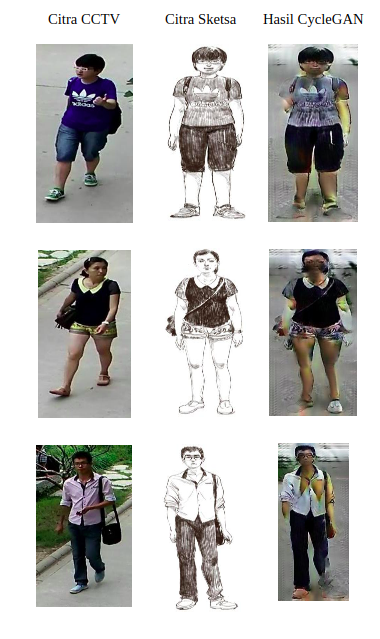
\includegraphics[scale=0.35]{img/CycleGANresults.png}
	\caption{Contoh hasil CycleGAN generasi ke 200}
	\label{fig: 3_3}
\end{figure}

Untuk CycleGAN nya sendiri, kami menggunakan model yang dibuat oleh Jun-Yan Zhu et al. dengan \textit{pre-trained weights} milik \textit{facades\_label2photo}. Citra yang digunakan untuk melatih gambar ini merupakan 600 citra yang terdapat pada dataset PKU Sketch Re-ID, dimana model ini di inisialisasi dengan \textit{learning rate} sebesar 0.0002 dan menurun ke 0.0001 setelah 150 epochs. Model CycleGAN ini kami \textit{train} selama 1000 epoch, namun kami memilih generasi ke 200 untuk dataset kami dikarenakan hasil sudah cukup baik.

\section{\textit{Local Binary Pattern}}
\vspace{1ex}
Salah satu cara lain yang kami gunakan untuk menjembatani perbedaan modalitas yang dimiliki oleh citra CCTV dan citra sketsa merupakan penggunaan \textit{Local Binary Pattern}. Dengan menggunakan \textit{Local Binary Pattern} dapat dilakukan pengambilan fitur tekstur dari citra CCTV, selain itu \textit{Local Binary Pattern} juga menggunakan citra hitam putih sehingga menyerupai citra sketsa yang ada.

\section{\textit{Training} dan \textit{Testing}}
\vspace{1ex}

\begin{figure}[h!] \centering
	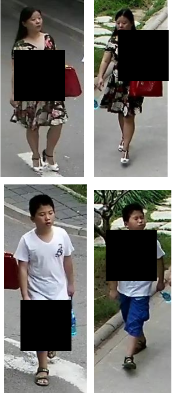
\includegraphics[width=0.28\textwidth]{img/RandomErasing.png}
	\caption{Contoh dari Random Erasing}
	\label{fig:4}
\end{figure}

Untuk memastikan bahwa kinerja model yang digunakan dapat diandalkan, kami melakukan proses training dan testing sebanyak 10 kali dan mengambil nilai rata-ratanya sebagai metrik evaluasi \textit{final}. Semua metode dievaluasi menggunakan akurasi Rank-1 milik model masing-masing, mengikuti ketentuan evaluasi yang ditentukan oleh Lu Pang et al.

\pagebreak

Pada eksperimen kami, kami mengatasi kurangnya data pada dataset PKU Sketch Re-Identification dengan cara melakukan \textit{pre-training} pada dataset Market-1501. Proses \textit{training} dilakukan selama 100 \textit{epochs}, dimana \textit{training} di inisialisasi dengan \textit{learning rate} sebesar 0,1 . \textit{Learning rate} tersebut akan berkurang dengan faktor  0.1 setiap 40 \textit{epochs}. Selain itu, kami melakukan \textit{random erasing} dan \textit{random crop} untuk menambahkan lebih banyak data \textit{training}. Gambar \ref{fig:4} menunjukan beberapa contoh dari augmentasi data yang dilakukan dengan metode \textit{Random Erasing}.

\section{Studi Ablasi}
\vspace{1ex}
Untuk memaksimalkan performa dari model ResNet-CIFAR yang digunakan, dilakukan studi ablasi dengan cara mengubah ukuran \textit{Fully Connected Layer} pertama yang digunakan oleh model. Ukuran \textit{Fully Connected Layer} yang digunakan adalah sebagai berikut; FC-128, FC-256, FC-512, FC-768, dan FC-1024. Selain itu dilakukan studi ablasi kedua dengan cara merubah probabilitas Random Erasing dari 0\% hingga 50\%. Pada pengujian ini kami hanya menggunakan model ResNet 56 dan ResNet 110 dikarenakan pada eksperimen sebelumnya kedua model tersebut mendapatkan rank-1 accuracy tertinggi dan kedua tertinggi.

\pagebreak
